\documentclass[final, 20pt]{beamer}
% poster
\usepackage[size=custom, width=121.92, height=91.44]{beamerposter}
% common stuff
\usepackage{graphicx}
\usepackage{hyperref}
\usepackage{booktabs}
\usepackage{amsmath}
\usepackage{caption}
\usepackage{subcaption}
\usepackage{enumitem}
\usepackage{array}
\usepackage{xparse}
% font
\usefonttheme{serif}
\setbeamerfont{block title}{size=\Large, series=\bfseries}
\setbeamerfont{headline title}{size=\fontsize{96}{0pt}\selectfont, series=\bfseries}
\setbeamerfont{headline author}{size=\large, series=\bfseries}
% main color
\definecolor{theme-1}{HTML}{2155CD} % #2155CD
\definecolor{theme-2}{HTML}{0AA1DD} % #0AA1DD
\definecolor{theme-3}{HTML}{79DAE8} % #79DAE8
\definecolor{theme-4}{HTML}{E8F9FD} % #E8F9FD
% set color
\setbeamercolor{block title}{fg=white, bg=theme-2}
\setbeamercolor{headline title}{fg=white, fg=theme-2}
% linespace
\usepackage{setspace}
\setstretch{1.25}
% size
\setlength{\paperwidth}{48in}
\setlength{\paperheight}{36in}
\newlength{\sepwidth}
\newlength{\colwidth}
\newlength{\twocolwidth}
\newlength{\contentwidth}
\newlength{\contentheight}
\newlength{\marginwidth}

\usepackage{calc}
\setlength{\marginwidth}{1in}
\setlength{\contentwidth}{\paperwidth - 2\marginwidth}
\setlength{\contentheight}{\paperheight - 3in}
\setlength{\sepwidth}{0.005\contentwidth}
% 4 columns
\setlength{\colwidth}{(\contentwidth - 3\sepwidth) / 4}
\setlength{\twocolwidth}{\colwidth + \sepwidth + \colwidth}
% empty spacer column
\NewDocumentCommand{\separatorcolumn}{}{\begin{column}{\sepwidth}\end{column}}
\NewDocumentCommand{\margincolumn}{}{\begin{column}{\marginwidth}\end{column}}
% top head template
\setbeamertemplate{headline}{
  \begin{beamercolorbox}{headline}
    \usebeamerfont{headline}
    \vskip1.5in
    \centering
    {\usebeamerfont{headline title}\usebeamercolor[fg]{headline title}\inserttitle\\[0.5ex]}
    {\usebeamerfont{headline author}\usebeamercolor[fg]{headline author}\insertauthor\\[1ex]} % author is not allowed.
    \ifbeamercolorempty[bg]{headline rule}{}{
      \begin{beamercolorbox}[wd=\paperwidth,colsep=0.5ex]{headline rule}\end{beamercolorbox}
    }
  \end{beamercolorbox}
}
\usepackage{tikz}
\usetikzlibrary{calc}
\NewDocumentCommand{\ensuremargin}{}{
  \begin{tikzpicture}[remember picture,overlay]
    \draw[black] ($(current page.north west) - (0, 1.5in)$) -- ($(current page.north east) - (0, 1.5in)$);
    \draw[black] ($(current page.south west) + (0, 1.5in)$) -- ($(current page.south east) + (0, 1.5in)$);
    \draw[black] ($(current page.north west) + (1in, 0)$) -- ($(current page.south west) + (1in, 0)$);
    \draw[black] ($(current page.north east) - (1in, 0)$) -- ($(current page.south east) - (1in, 0)$);
  \end{tikzpicture}
}
% header helper
\usepackage{xhfill}
\NewDocumentCommand{\header}{m O{1.5em}}{\vspace{#2}\begingroup\usebeamercolor[bg]{block title}\scshape\large#1\par\vspace{-0.55\baselineskip}\hrulefill\endgroup}
\NewDocumentCommand{\subheader}{m}{\begingroup\usebeamercolor[bg]{block title}\bfseries#1\par\endgroup}

% multicol
\usepackage{multicol}
% hanging indent
\usepackage{hanging}
% color
\setbeamercolor{block title}{fg=white, bg=theme-2}
% numbered figure and table
\setbeamertemplate{caption}[numbered]
% metadata
\title{Wireless Online Real-time Language Expression Yielder}
\author{Anish Goyal \& Ian Oberbeck \& Yubo Cao\\\normalfont\selectfont GOSA Governor's Honors Program 60 Engineering}
% bullet
\setlist[itemize]{leftmargin=0.5em, label=\usebeamercolor[bg]{block title}\textbullet}
% redefine block
\let\block=\undefined
\let\endblock=\undefined
\usepackage[most]{tcolorbox}
\newtcolorbox{block}[1]{enhanced, colback=white, colframe=theme-2!50, colbacktitle=theme-2, coltitle=white, fonttitle=\bfseries, title=\Large#1, boxrule=1pt, boxsep=1.5em, breakable, sharpish corners, bottomrule=0.5em, toptitle=-0.75em, bottomtitle=-0.75em}
% microtype
\usepackage[activate={true,nocompatibility},final]{microtype}

% remove navigation
\setbeamertemplate{navigation symbols}{}
% make vfill work in beamer columns
\usepackage{etoolbox}
\let\oldcolumn\column
\let\oldendcolumn\endcolumn
\RenewDocumentEnvironment{column}{m O{\contentheight - 2.7in}}{%
  \oldcolumn{#1}%
  \minipage[c][#2][s]{\columnwidth}
}{\endminipage\oldendcolumn}

\begin{document}

\begin{frame}[t]
  \centering
  \begin{columns}[t]
    \margincolumn

    \begin{column}{\colwidth}
      \begin{block}{Research Question}
        \header{Problem}[0pt]

        The ship's performance, measured by total resistance coefficient, $C_T$, is significantly affected by the geometry of the ship hull. The design of a ship hull though, is usually not fully evaluated during the design stage, until production and testing (Birk, 2019). However, it is crucial to make changes to ship hull shape to increase efficiency. For instance, by using a more efficient design, fuel savings ranging from 25\% to 75\% can be accomplished. Traditional methods for evaluating hull resistance, such as experimental testing and empirical formulas, can be time-consuming and costly, and may not always provide accurate results.

        \header{Existing Solution}[2cm]

        \begin{description}
          \item[Holtrop and Mennen Method] empirical formula used to estimate the total resistance of a ship's hull using the dimensions and other characteristics of the hull. It is used as a quick and simple way to estimate a ship's resistance without the need for costly and time-consuming experimental or computational tests. However, it still requires at least six coefficients and is only valid for a limited range of ship dimensions.
          \item[COMSOL] a computational fluid dynamics (CFD) simulations to model the flow of water around the hull and calculate the resulting drag and other types of resistance (COMSOL, n.d.). Huge amount of computational power is required to run the simulation, and the results are not always accurate.
        \end{description}

        \header{Research Question}[2cm]

        How does the curvature of the ship hull, measured by RMSE-roundness (root mean square error roundness), affect the performance of the ship, as measured by the total resistance coefficient?
      \end{block}

      \vfill

      \begin{block}{Hypothesis}
        \header{Hypothesis}[0pt]

        The ship's performance, measured by total resistance coefficient ($C_T$) decreases as the RMSE-roundness of the ship hull increases.

        \header{Justification}[2cm]

        A ship hull with a gentle curvature and a smooth, streamlined shape may create a thin boundary layer that allows the fluid to flow smoothly, reducing the total resistance experienced by the ship and improving its performance. In contrast, a ship hull with a sharp curvature or a rough or irregular shape may create a thick boundary layer that disrupts the flow of fluid, increasing the total resistance experienced by the ship and reducing its performance.

        \header{Null Hypothesis}[2cm]

        RMSE-roundness of the ship hull has no effect on the ship’s performance, $C_T$.
      \end{block}
    \end{column}

    \separatorcolumn

    \begin{column}{\twocolwidth}
      \begin{block}{Methods}

        \setlength{\columnsep}{2em}
        \begin{multicols}{2}
          \header{Modelling}[0pt]

          \begin{itemize}
            \item Collect ship hull models online
            \item Export the models to \texttt{.stl} format and print them using a Stratasys 170 3D printer
            \item Create hooks on the hulls to attach them to the force sensor
          \end{itemize}

          \begin{minipage}[t]{0.48\linewidth}
            \subheader{Control}

            ship hulls with a nearly zero RMSE-roundness

            \centering
            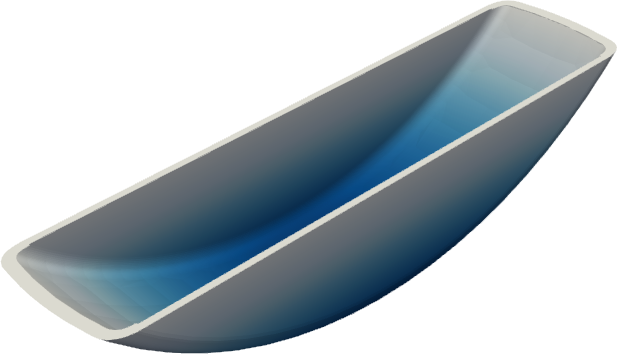
\includegraphics[width=0.4\linewidth]{images/control.png}
          \end{minipage}{\hspace*{0.75em}\color{theme-2!50}\vline\hspace*{0.5em}}
          \begin{minipage}[t]{0.48\linewidth}
            \subheader{Experiment}

            ship hulls with different RMSE-roundness

            \centering
            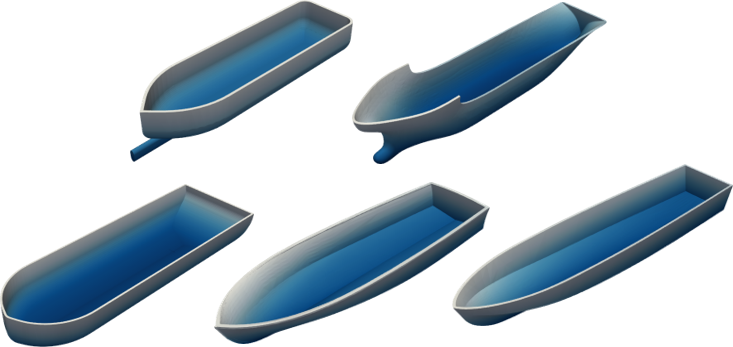
\includegraphics[width=0.5\linewidth]{images/experiment-ship-hulls.png}
          \end{minipage}


          \header{Independent Variable}[0.5em]

          RMSE roundness is the independent variable.
          \begin{equation}
            \label{eq:rmse}
            RMSE = \sqrt{\frac{1}{n}\sum_{i=1}^{n}(x_i - \bar{x})^2}
          \end{equation}
          where $n$ is the number of points, $x_i$ is the $i$th point of the hull line and $\bar{x}$ is the best-fit circle  of the hull line predicted point.


          \header{Experimentation}[0.5em]

          \begin{itemize}
            \item Connect a force sensor with a rope at each side, and connect the rope to the hook on the ship hull. Measure and record the temperature, atmospheric pressure, and mass of the ship hull and the ballast.
            \item Drag the ship hulls for 3 seconds and record data at 20 Hz
            \item Measure and record the temperature of liquid and distance travelled by the researcher.
          \end{itemize}

          \begin{figure}
            \centering
            \begin{subfigure}[b]{0.48\linewidth}
              \centering
              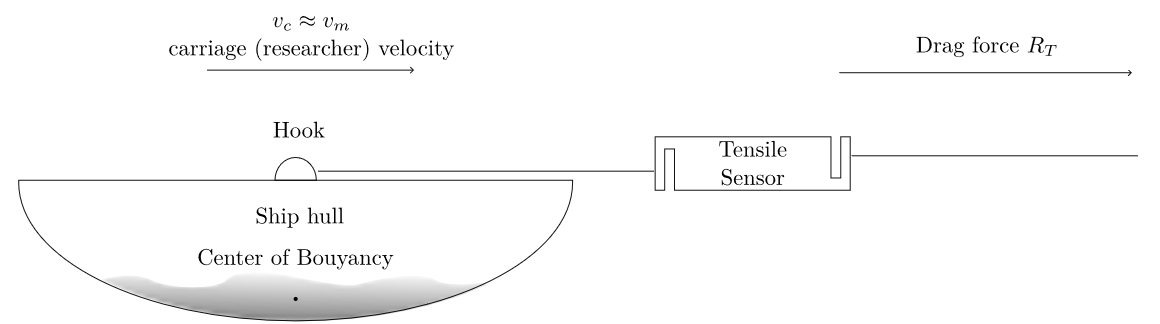
\includegraphics[width=\linewidth]{images/symbolic-setup}
              \caption{Symbolic representation of the setup}
            \end{subfigure}
            \begin{subfigure}[b]{0.48\linewidth}
              \centering
              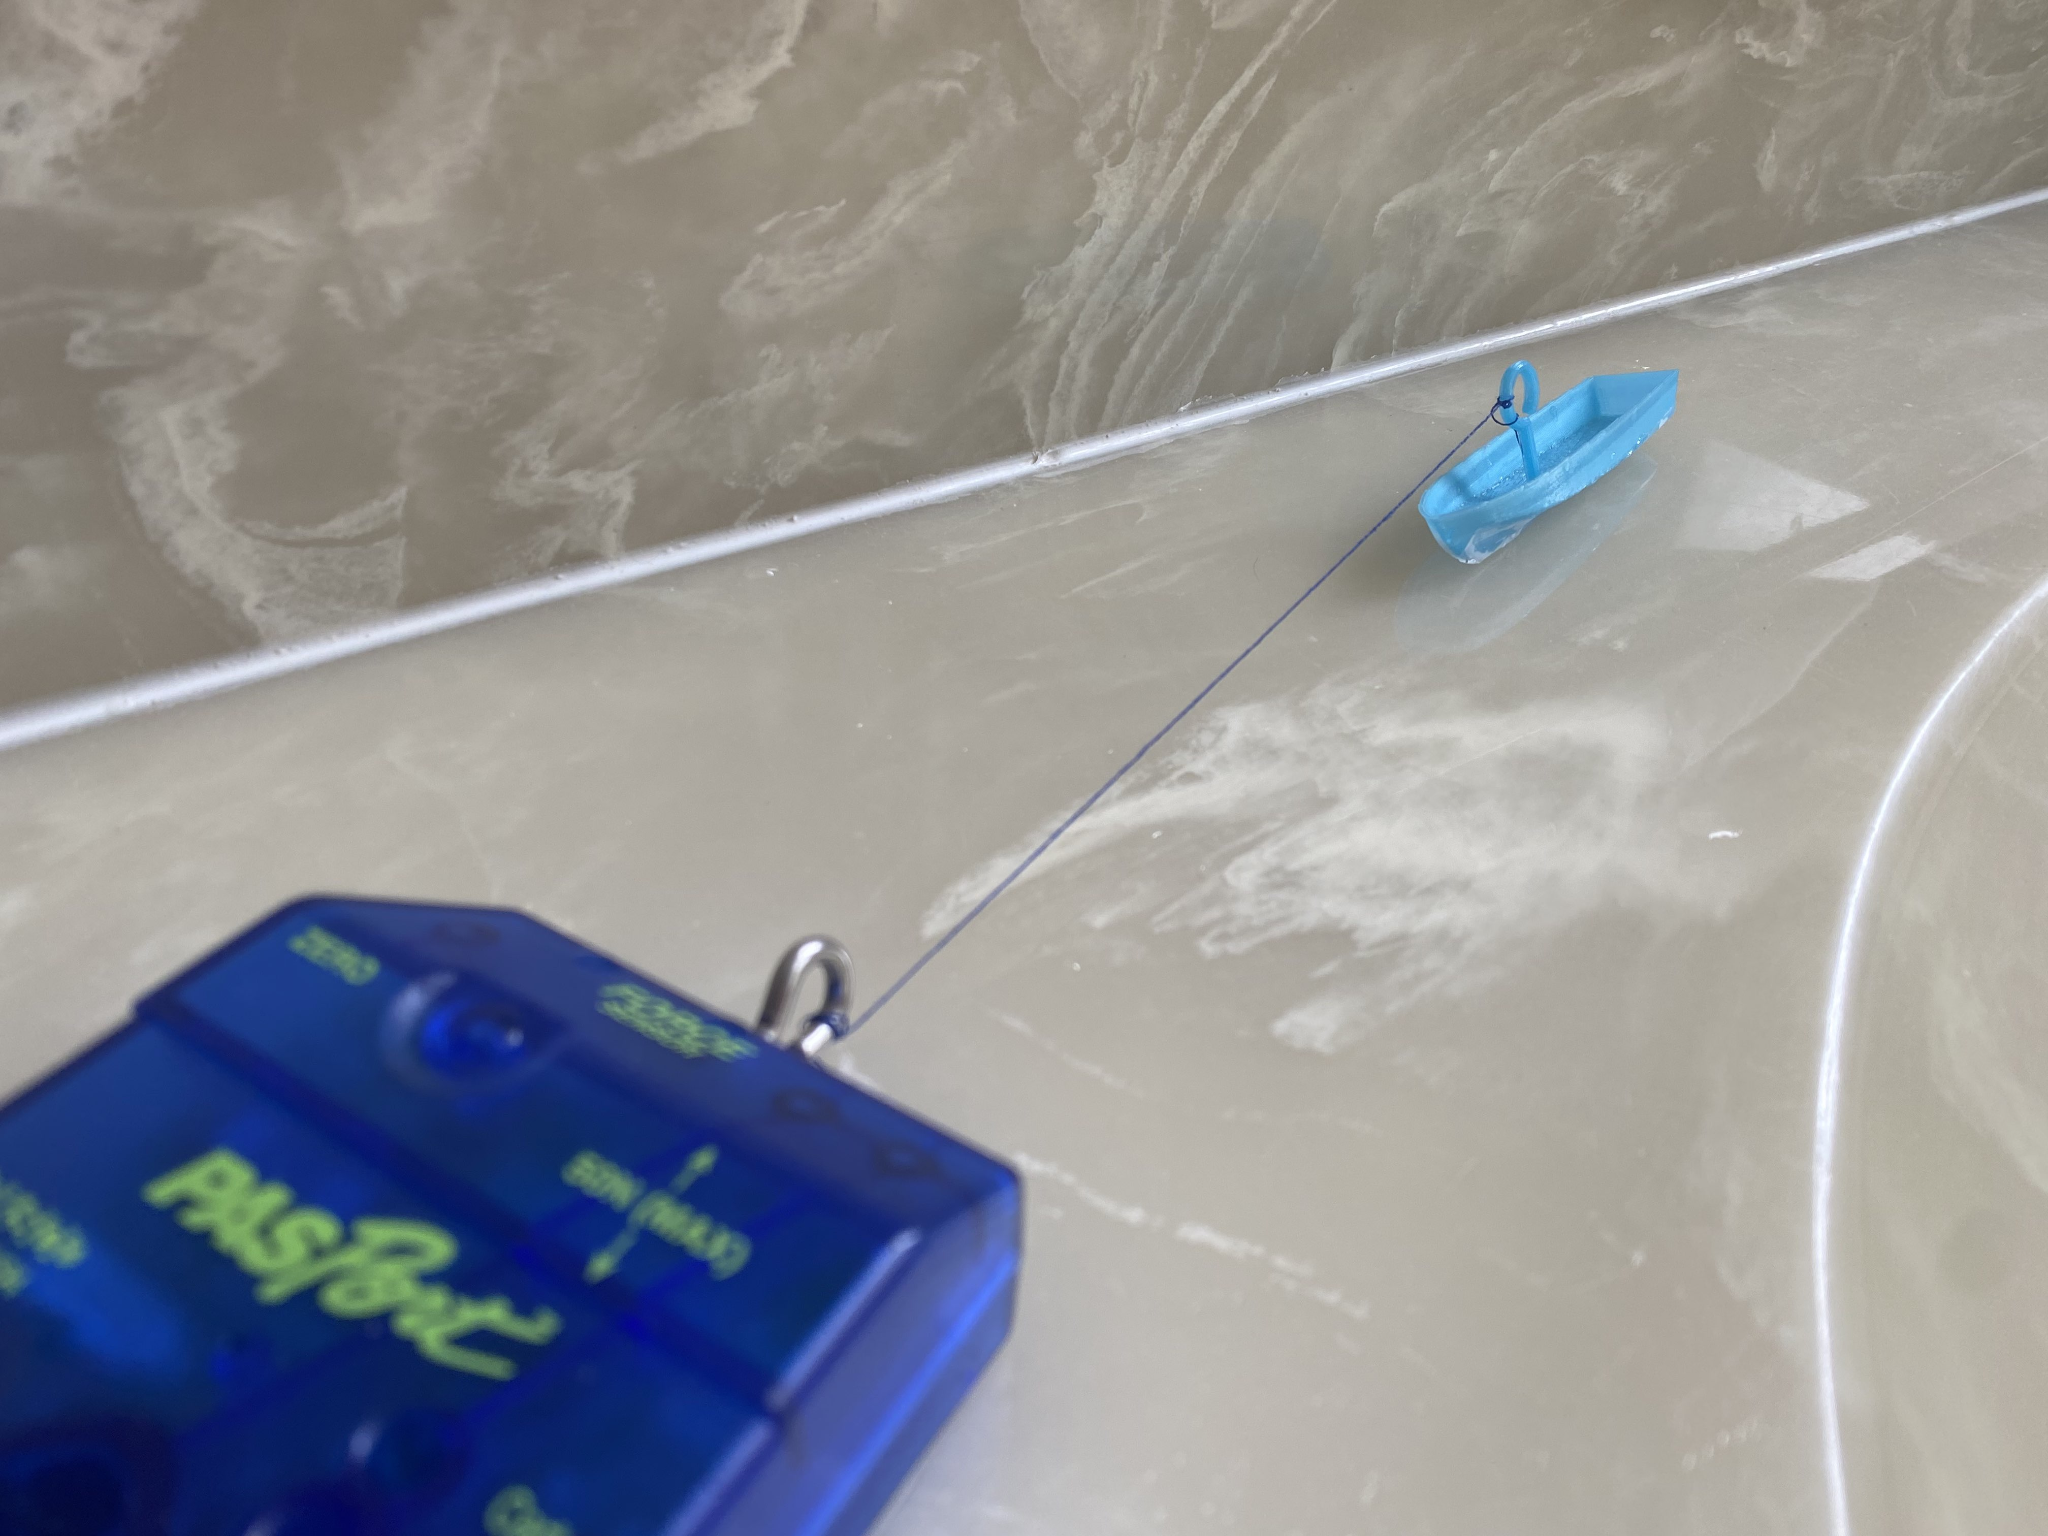
\includegraphics[width=0.5\linewidth]{images/experiment-setup}
              \caption{Researchers conducting the experiment}
            \end{subfigure}
            \caption{Experiment Setup}
          \end{figure}

          \header{Dependent Variable}[0pt]

          Calculate the total resistance coefficient, $C_T$, using the following equation:
          \begin{equation}
            \label{eq:ct}
            C_T = \frac{F}{\frac{1}{2} \rho V^2 S}
          \end{equation}
          where $F$ is the force measured by the force sensor, $\rho$ is the density of the water, $V$ is the velocity of the ship hull, and $S$ is the wet surface area of the ship hull
        \end{multicols}
      \end{block}

      \vfill

      \begin{block}{Result}
        \begin{minipage}[c]{0.48\linewidth}
          \begin{figure}
            \centering
            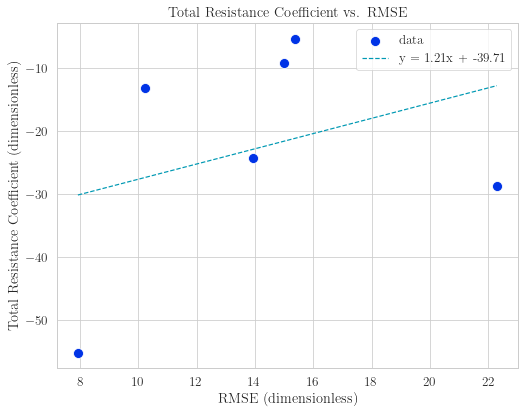
\includegraphics[width=0.65\linewidth]{images/total-resistance-coefficient-vs-rmse}
            \caption{The total resistance coefficient of the ship hull ($C_T$) versus the RMSE-roundness of the ship hull. A weak, positive linear relationship exists.}
          \end{figure}
        \end{minipage}
        \begin{minipage}[c]{0.48\linewidth}
          \begin{table}
            \begin{tabular}{c*{2}{>{\centering\arraybackslash}p{0.3\linewidth}}}
              \toprule
              \textbf{Ship hull} & \textbf{RMSE-roundness (dimensionless)} & \textbf{Total Resistance Coefficient $C_T$ } \\
              \midrule
              control            & 7.9                                     & -75                                          \\
              ship hull 3        & 10                                      & -13                                          \\
              ship hull 5        & 14                                      & -53                                          \\
              ship hull 2        & 15                                      & -9.2                                         \\
              ship hull 1        & 15                                      & -4.8                                         \\
              ship hull 4        & 22                                      & -29                                          \\
              \bottomrule
            \end{tabular}
            \caption{The total resistance coefficient ($C_T$) and RMSE-roundness of each ship hull}
          \end{table}
        \end{minipage}
      \end{block}

      \vfill

      \begin{block}{Interpretation}
        \setlength{\columnsep}{2em}
        \begin{multicols}{2}
          \header{Normal Distribution}

          \begin{figure}
            \centering
            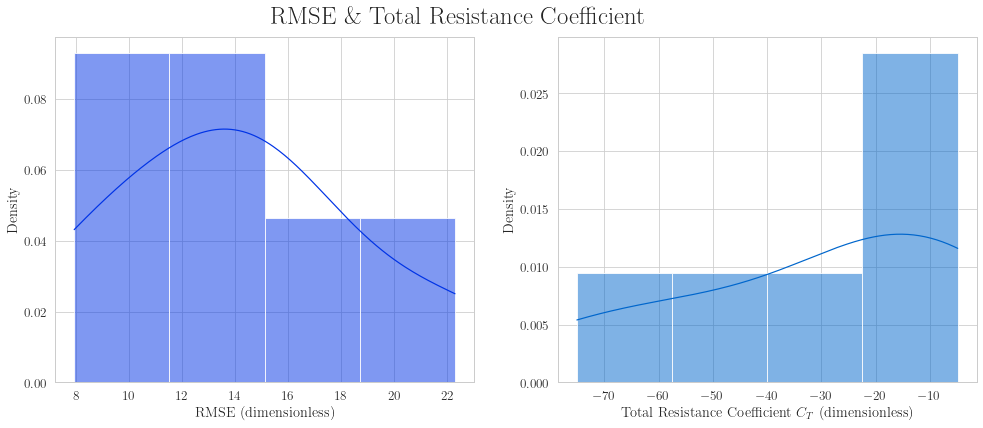
\includegraphics[width=0.8\linewidth]{images/rmse-vs-ct-histplot}
            \caption{Histgram of $C_T$ and RMSE-roundness}
          \end{figure}

          \begin{description}
            \item[RMSE-roundness] Statistic: $0.95$, P-value: $0.71$
            \item[Total resistance coefficient] Statistic: $0.89$, P-value: $0.31$
          \end{description}

          Both the RMSE-roundness and total resistance coefficient variables are not normally distributed, as p-values for both variables are greater than $0.05$.

          \columnbreak

          \header{Correlation}

          Hence, non-parametric tests are used to determine the correlation between the two variables.

          \begin{description}
            \item[Spearman] P-value = $0.27$, correlation coefficient = $0.54$
            \item[Kendall Tau] P-value = $0.27$, correlation coefficient = $0.57$
          \end{description}

          The probability of the correlation is $0.27$ and $0.26$. Based on these values, it is not possible to reject the null hypothesis. The correlation coefficient is $0.54$ and $0.57$. These values indicate a weak and positive linear relationship between the two variables.
        \end{multicols}
      \end{block}
    \end{column}

    \separatorcolumn

    \begin{column}{\colwidth}
      \begin{block}{Conclusions}
        There is no statistical correlation ($0.27 > 0.05$) between the RMSE-roundness of the ship hull and the total resistance coefficient, concluded with the low correlation values calculate ($0.54 < 0.95$). However, a weak and positive linear relationship exists between the two variables from interpretation of correlation coefficients. This experiment disproves the conventional wisdom that ship hulls with higher roundness will encounter lower overall resistance.
      \end{block}

      \vfill

      \begin{block}{Application}
        \begin{itemize}
          \item The rejection of RMSE-roundness as a variable in the optimization of ship hulls.
          \item Further investigation and use of the innovative method of measuring curvature in data gathering and model development.
          \item Improved understanding of the factors that impact the resistance of ship hulls and the potential for reducing resistance and improving performance.
          \item Development of more effective design and optimization techniques for ship hulls.
          \item Guiding future research to consider using larger, more realistic ship hull models and more accurate testing environments in order to avoid the limitations of the current study.
        \end{itemize}
      \end{block}

      \vfill

      \begin{block}{Limitation}
        \begin{itemize}
          \item The extremely small size of the ship hulls tested made it difficult to obtain accurate measurements.
          \item The precision of the instrument used for measuring total resistance may have been inadequate.
          \item It was impossible to maintain a constant speed of dragging during the experiments.
          \item The limited distance that could be covered by dragging the ship hulls may have impacted the reliability of the results.
          \item The low resistance force measured made it difficult to detect statistical differences between the data from different ship hulls.
        \end{itemize}

        These limitations may have affected the accuracy and reliability of the study's conclusions.
      \end{block}

      \vfill

      \begin{block}{References}
        \setstretch{1.8}
        \tiny
        \begin{multicols}{2}

          \begin{hangparas}{0.5in}{1}
            Birk, L. (2019). Fundamentals of ship hydrodynamics: Fluid mechanics, ship resistance, and propulsion. John Wiley \& Sons Ltd. \url{https://onlinelibrary.wiley.com/doi/book/10.1002/9781119191575}

            Bullock, R. (2017, February 12). Least-Squares Circle Fit. Documentation. Retrieved September 14, 2022, from \url{https://dtcenter.org/community-code/model-evaluation-tools-met/documentation}

            Engineering ToolBox. (2003). Water---density, specific weight, and thermal expansion coefficients. \url{https://www.engineeringtoolbox.com/water-density-specific-weight-d_595.html}

            IITC. (2017). Ship models. International towing tank Conference recommended procedures and guidelines. \url{https://www.ittc.info/media/7975/75-01-01-01.pdf}

            IITC. (2021). Resistance test. International towing tank Conference recommended procedures and guidelines. \url{http://www.ittc.info/media/9595/75-02-02-01.pdf}

            Lin, J.-f., Zhao, D.-g., Guo, C.-y., Su, Y.-m., \& Zhong, X.-h. (2020).

            GrabCAD. (n.d.). Grabcad making additive manufacturing at scale possible. GrabCAD Making Additive Manufacturing at Scale Possible. Retrieved September 14, 2022, from https://grabcad.com/

            Lin, J.-feng, Zhao, D.-gang, Guo, C.-yu, Su, Y.-min, \& Zhong, X.-hai. (2020). Comprehensive test system for ship-model resistance and propulsion performance in Actual seas. Ocean Engineering, 197, 106915. \url{https://doi.org/10.1016/j.oceaneng.2019.106915}

            International Association for the Properties of Water and Steam, IAPWS R6-95 (2018), Revised Release on the IAPWS Formulation 1995 for the Thermodynamic Properties of Ordinary Water Substance for General and Scientific Use (2018)
          \end{hangparas}
        \end{multicols}

      \end{block}
    \end{column}

    \margincolumn
  \end{columns}

  \tikz {
    \draw ($(current page.south west)!0.5!(current page.south east)$) node {All charts, graphs, photos, and diagrams are the product of the student researcher.};
    
  }
\end{frame}
\end{document}

